% Options for packages loaded elsewhere
\PassOptionsToPackage{unicode}{hyperref}
\PassOptionsToPackage{hyphens}{url}
\PassOptionsToPackage{dvipsnames,svgnames*,x11names*}{xcolor}
%
\documentclass[
  11pt,
  krantz2, a4paper, twoside]{krantz}
\usepackage{amsmath,amssymb}
\usepackage{lmodern}
\usepackage{setspace}
\usepackage{ifxetex,ifluatex}
\ifnum 0\ifxetex 1\fi\ifluatex 1\fi=0 % if pdftex
  \usepackage[T1]{fontenc}
  \usepackage[utf8]{inputenc}
  \usepackage{textcomp} % provide euro and other symbols
\else % if luatex or xetex
  \usepackage{unicode-math}
  \defaultfontfeatures{Scale=MatchLowercase}
  \defaultfontfeatures[\rmfamily]{Ligatures=TeX,Scale=1}
  \setmainfont[]{NanumMyeongjo}
\fi
% Use upquote if available, for straight quotes in verbatim environments
\IfFileExists{upquote.sty}{\usepackage{upquote}}{}
\IfFileExists{microtype.sty}{% use microtype if available
  \usepackage[]{microtype}
  \UseMicrotypeSet[protrusion]{basicmath} % disable protrusion for tt fonts
}{}
\makeatletter
\@ifundefined{KOMAClassName}{% if non-KOMA class
  \IfFileExists{parskip.sty}{%
    \usepackage{parskip}
  }{% else
    \setlength{\parindent}{0pt}
    \setlength{\parskip}{6pt plus 2pt minus 1pt}}
}{% if KOMA class
  \KOMAoptions{parskip=half}}
\makeatother
\usepackage{xcolor}
\IfFileExists{xurl.sty}{\usepackage{xurl}}{} % add URL line breaks if available
\IfFileExists{bookmark.sty}{\usepackage{bookmark}}{\usepackage{hyperref}}
\hypersetup{
  pdftitle={신약개발을 위한 실전 약동학 (I - 이론과 자료해석)},
  pdfauthor={Ver. 20210208},
  colorlinks=true,
  linkcolor=Maroon,
  filecolor=Maroon,
  citecolor=Blue,
  urlcolor=Blue,
  pdfcreator={LaTeX via pandoc}}
\urlstyle{same} % disable monospaced font for URLs
\usepackage{longtable,booktabs,array}
\usepackage{calc} % for calculating minipage widths
% Correct order of tables after \paragraph or \subparagraph
\usepackage{etoolbox}
\makeatletter
\patchcmd\longtable{\par}{\if@noskipsec\mbox{}\fi\par}{}{}
\makeatother
% Allow footnotes in longtable head/foot
\IfFileExists{footnotehyper.sty}{\usepackage{footnotehyper}}{\usepackage{footnote}}
\makesavenoteenv{longtable}
\setlength{\emergencystretch}{3em} % prevent overfull lines
\providecommand{\tightlist}{%
  \setlength{\itemsep}{0pt}\setlength{\parskip}{0pt}}
\setcounter{secnumdepth}{5}
%\usepackage{tikz-cd} % \xleftrightarrow
%\usepackage{amsmath} 
%\documentclass[b5paper,9pt]{extarticle}
%\usepackage{geometry}

%\usepackage[%
%  b5, % <===============================================================
%  center, cam
%  %axes,cross,pdftex,center
%]{crop}

%sungpil defined above

\usepackage{booktabs}
\usepackage{longtable}
\usepackage[bf,singlelinecheck=off]{caption}

%\usepackage[utf8]{inputenc}

%\usepackage{xeCJK}
%\setCJKmainfont[$for(CJKoptions)$$CJKoptions$$sep$,$endfor$]{$CJKmainfont$}

%\usepackage{xeCJK}
%\setCJKmainfont{SimSun}

%\usepackage{xeCJK}
%\setCJKmainfont{SimSun}
%\setmainfont{Calibri}
%\setCJKmainfont{宋体}

%\setmainhanjafont{SimSun}
%\setmainfont[UprightFeatures={SmallCapsFont=AlegreyaSC-Regular}]{Alegreya}

%\setmainhanjafont[
%  BoldFont=*, BoldFeatures={FakeBold=2},
%  ItalicFont=*, ItalicFeatures={FakeSlant=0.17},
%  SlantedFont=*, SlantedFeatures={FakeSlant=0.17},
%  BoldItalicFont=*, BoldItalicFeatures={FakeBold=2,FakeSlant=0.17},
%  BoldSlantedFont=*, BoldSlantedFeatures={FakeBold=2,FakeSlant=0.17},
%]{SimSun}

\usepackage{framed,color}
\definecolor{shadecolor}{RGB}{248,248,248}

\renewcommand{\textfraction}{0.05}
\renewcommand{\topfraction}{0.8}
\renewcommand{\bottomfraction}{0.8}
\renewcommand{\floatpagefraction}{0.75}

\renewenvironment{quote}{\begin{VF}}{\end{VF}}
\let\oldhref\href
\renewcommand{\href}[2]{#2\footnote{\url{#1}}}

\ifxetex
  \usepackage{letltxmacro}
  \setlength{\XeTeXLinkMargin}{1pt}
  \LetLtxMacro\SavedIncludeGraphics\includegraphics
  \def\includegraphics#1#{% #1 catches optional stuff (star/opt. arg.)
    \IncludeGraphicsAux{#1}%
  }%
  \newcommand*{\IncludeGraphicsAux}[2]{%
    \XeTeXLinkBox{%
      \SavedIncludeGraphics#1{#2}%
    }%
  }%
\fi

\makeatletter
\newenvironment{kframe}{%
\medskip{}
\setlength{\fboxsep}{.8em}
 \def\at@end@of@kframe{}%
 \ifinner\ifhmode%
  \def\at@end@of@kframe{\end{minipage}}%
  \begin{minipage}{\columnwidth}%
 \fi\fi%
 \def\FrameCommand##1{\hskip\@totalleftmargin \hskip-\fboxsep
 \colorbox{shadecolor}{##1}\hskip-\fboxsep
     % There is no \\@totalrightmargin, so:
     \hskip-\linewidth \hskip-\@totalleftmargin \hskip\columnwidth}%
 \MakeFramed {\advance\hsize-\width
   \@totalleftmargin\z@ \linewidth\hsize
   \@setminipage}}%
 {\par\unskip\endMakeFramed%
 \at@end@of@kframe}
\makeatother

\makeatletter
\@ifundefined{Shaded}{
}{\renewenvironment{Shaded}{\begin{kframe}}{\end{kframe}}}
\makeatother

\newenvironment{rmdblock}[1]
  {
  \begin{itemize}
  \renewcommand{\labelitemi}{
    \raisebox{-.7\height}[0pt][0pt]{
      {\setkeys{Gin}{width=3em,keepaspectratio}\includegraphics{images/#1}}
    }
  }
  \setlength{\fboxsep}{1em}
  \begin{kframe}
  \item
  }
  {
  \end{kframe}
  \end{itemize}
  }
\newenvironment{rmdnote}
  {\begin{rmdblock}{note}}
  {\end{rmdblock}}
\newenvironment{rmdcaution}
  {\begin{rmdblock}{caution}}
  {\end{rmdblock}}
\newenvironment{rmdimportant}
  {\begin{rmdblock}{important}}
  {\end{rmdblock}}
\newenvironment{rmdtip}
  {\begin{rmdblock}{tip}}
  {\end{rmdblock}}
\newenvironment{rmdwarning}
  {\begin{rmdblock}{warning}}
  {\end{rmdblock}}

\usepackage{makeidx}
\makeindex

\urlstyle{tt}

%https://tex.stackexchange.com/questions/85400/how-to-change-space-around-theorem-environments

\usepackage{amsthm}
\makeatletter
\def\example@space@setup{%
  \example@preskip=0.001cm
  \example@postskip=\thm@preskip
}
\makeatother

%https://github.com/rstudio/bookdown/issues/901
\usepackage{caption}
\captionsetup[figure]{labelsep=period}
\captionsetup[table]{labelsep=period}

\frontmatter
\usepackage{kotex}
\usepackage{chemarr}
\usepackage{booktabs}
\usepackage{longtable}
\usepackage{array}
\usepackage{multirow}
\usepackage{wrapfig}
\usepackage{float}
\usepackage{colortbl}
\usepackage{pdflscape}
\usepackage{tabu}
\usepackage{threeparttable}
\usepackage{threeparttablex}
\usepackage[normalem]{ulem}
\usepackage{makecell}
\usepackage{xcolor}
\ifluatex
  \usepackage{selnolig}  % disable illegal ligatures
\fi

\title{신약개발을 위한 실전 약동학 (I - 이론과 자료해석)}
\author{Ver. 20210208}
\date{Ver. 20210208}

\begin{document}
\maketitle

%\cleardoublepage\newpage\thispagestyle{empty}\null
%\cleardoublepage\newpage\thispagestyle{empty}\null
%\cleardoublepage\newpage

\newpage

\thispagestyle{empty}

\begin{center}

\includegraphics{images/pipet.pdf}
\end{center}

\thispagestyle{empty}
%\scriptsize
%\hfill Ver. 20200801
%\normalsize
\begin{center}
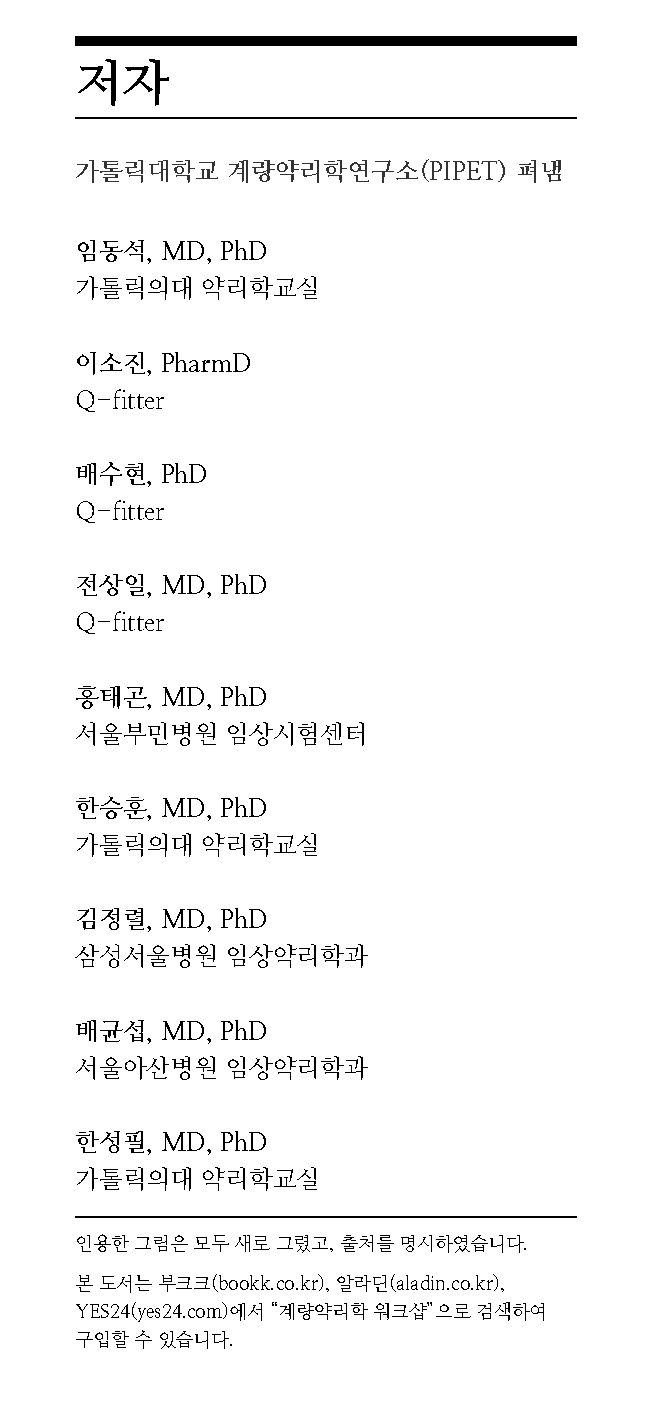
\includegraphics{images/authors.pdf}
\end{center}

\setlength{\abovedisplayskip}{-5pt}
\setlength{\abovedisplayshortskip}{-5pt}

\newpage\thispagestyle{empty}\null

{
\hypersetup{linkcolor=}
\setcounter{tocdepth}{2}
\tableofcontents
}
\setstretch{1.30}
\hypertarget{uxba38uxb9acuxb9d0}{%
\chapter*{머리말}\label{uxba38uxb9acuxb9d0}}


\normalsize

계량약리학은 신약개발 현장에서 제기되는 질문들에 대한 답을 정량적으로 찾아내기 위한 과정에서 정립되어온 학문입니다. 물론 계량약리학은 이미 허가된 약들의 적절한 용법을 찾는 데에도 쓸 수 있지만, 신약개발이라는 큰 목표를 빼고서는 이 어려운 방법론을 배워야 할 이유를 찾기는 힘듭니다. 우리나라의 신약개발은 짧은 역사 속에서 많은 시행착오를 통해 발전해가고 있습니다. 국내에서 계량약리학에 대한 수요가 이만큼이나마 늘어난 것은 2010년대 중반 이후 두드러지게 보이는 이 같은 분위기의 변화와 맞물려 있겠습니다.

혼합효과 모델링(mixed-effects modeling)은 신약개발과 임상시험, 시판허가 등의 주요 의사결정에 필수적으로 쓰이고 있는 계량약리학적 접근법의 핵심적인 기법으로서 그 기본개념을 익히는 것이 결코 쉽지 않습니다. 서울성모병원 임상약리과와 가톨릭대학교 계량약리학연구소(PIPET, Pharmacometrics Institute for Practical Education and Training)는 혼합효과 모델링 기법을 가르치는 PK/PD 워크샵을 2009년도부터 매년 개최해 왔습니다. 시작할 때부터 지금까지 정부나 기업의 어떤 도움이나 간섭없이 사막에 씨앗을 뿌리는 심정으로 매년 그 내용을 양적, 질적으로 보완하면서 basic-1, basic-2, intermediate-1, intermediate-2의 서로 연결되는 각 1.5일의 교육 과정으로 발전시켜 왔습니다. 이제 십여 년간 축적되어온 교육의 경험을 바탕으로, 국내에서 입문자들이 보다 쉽게 이해하고 따라갈 수 있도록 워크샵의 basic-1과 2의 강의, 실습내용을 고스란히 옮겨 담은 교재를 책으로 펴내게 되었습니다. 그리고 이 책에 실린 내용들에 상응하는 워크샵 슬라이드와 실습용 파일들은 웹\footnote{\url{http://pipet.or.kr/board/resources_list.asp}}에서 내려 받으실 수 있습니다. 그 자료들과 이 책으로 함께 공부한다면 따로 워크샵을 듣지 않고도 basic-1과 2의 내용을 따라갈 수 있을 것입니다.

PIPET의 구성원들은 우리말로 된 입문용 교재가 전무한 현실을 타개하기 위해 2016년도에 `비선형혼합효과 모델을 적용한 집단 PK/PD 분석입문'(Joel S Owen, Jill Fiedler-Kelly 공저)을 번역, 출간한 바 있습니다. 여기에 더하여 국내 연구자들의 손으로 직접 집필한 이 PK/PD 모델링 교재까지 나왔으므로, 스스로 공부할 수 있는 인프라가 완비되었다고 자부할 수 있게 되었습니다. 이 책을 사서 열심히 보실 분들 중에는 관련 분야의 대학원생들이 많을 것이므로 책 전체를 인터넷 상에 공개하여 내려 받을 수 있게 하였습니다.\footnote{\url{http://pipet.or.kr/books/pharmapk}} 또한, 동시에 출간하는 종이책의 경우에도 컬러 인쇄를 유지하며 책값을 복사비 수준으로 낮추기 위해, 기존의 알려진 출판사들을 피하여 인터넷 서점 등에서 print on demand로 주문할 수 있는 개인출판의 방식을 채택하였습니다. 각 장의 저자들은 모두 워크샵에서 강사로 활동해 주신 분들로서 자신이 맡은 시간에 해당하는 원고를 작성하였고, 워크샵에 포함된 부분은 아니지만 이론적인 일부분을 보완하기 위해 울산의대의 배균섭 교수님께서 한 장을 맡아 주셨습니다. 모아진 원고들에 대한 정리, 색인, 조판 과정에서 애써 주신 한성필, 한승훈 교수님께 감사드립니다. 지난 십여 년간 저희가 매년 개최해 온 워크샵들에 등록하여 열심히 익히고 질문을 해 주신 식약처와 제약/바이오 업계의 수많은 연구자분들, 전국의 대학원생들께 또한 감사드립니다. 참가자들의 귀중한 질문과 피드백이 없었다면 이 책은 완성될 수 없었을 것입니다.

학계의 PK/PD 전문가들이 우리나라의 신약개발에 기여하는 방법 중의 하나는 신약개발의 최전선에서 일하고 있는 제약/바이오 업계의 풀뿌리 연구자들에 대한 지속적인 교육과 훈련 기회를 제공하는 것입니다. 그러한 사명감으로 맨땅에서 시작한 이 코스를 지난 십 수년간 오늘의 수준으로 끌어올릴 수 있게 해 준, PIPET을 거쳐간 귀한 젊은 연구자들의 공헌에 깊이 감사드립니다. 이름난 분들을 초빙해서 청중을 모으고 신문에 내는 행사를 수십 번을 한들, 젊은이들의 앞날을 염려하고, 이들을 제대로 가르치겠다는 의지가 없다면 그저 남들에게 보여주기 위한 이벤트에 지나지 않습니다. 그런 곳에 사람과 돈이 몰릴지는 몰라도, 한편에서는 세상의 각광과는 무관하게 소신대로 제 갈 길을 가는 소수가 있기 마련입니다. 매년 열던 워크샵을 책으로 엮어 내는 이 번거로운 작업도 그런 소신을 실천하는 것이며, 한국의 신약개발을 위해 작은 밑거름이라도 된다면 저자들은 큰 보람을 느낄 것입니다.

\begin{center}
\includegraphics[width=1\linewidth]{images/preface} \end{center}

\normalsize

\mainmatter

\hypertarget{principle}{%
\chapter{약동학 이론}\label{principle}}

\Large\hfill

임동석
\normalsize

\hypertarget{uxc57duxb3d9uxd559-uxc774uxb860}{%
\section{약동학 이론}\label{uxc57duxb3d9uxd559-uxc774uxb860}}

\hypertarget{admeuxc640-uxc57duxb3d9uxd559}{%
\section{ADME와 약동학}\label{admeuxc640-uxc57duxb3d9uxd559}}

\hypertarget{uxc57duxbb3c-uxbd84uxd3ec-uxbaa8uxb378uxacfc-uxbd84uxd3ecuxc6a9uxc801}{%
\section{약물 분포 모델과 분포용적}\label{uxc57duxbb3c-uxbd84uxd3ec-uxbaa8uxb378uxacfc-uxbd84uxd3ecuxc6a9uxc801}}

\hypertarget{uxccaduxc18cuxc728uxc758-uxac1cuxb150uxacfc-uxc801uxc6a9}{%
\section{청소율의 개념과 적용}\label{uxccaduxc18cuxc728uxc758-uxac1cuxb150uxacfc-uxc801uxc6a9}}

\hypertarget{uxb2e4uxd68cuxd22cuxc5ec-pkuxc640-uxcd5cuxc885uxbc18uxac10uxae30}{%
\section{다회투여 PK와 최종반감기}\label{uxb2e4uxd68cuxd22cuxc5ec-pkuxc640-uxcd5cuxc885uxbc18uxac10uxae30}}

\hypertarget{uxc815uxb9e5uxc8fcuxc785uxacfc-uxacbduxad6cuxd22cuxc5ec-pkuxc758-uxbe44uxad50}{%
\section{정맥주입과 경구투여 PK의 비교}\label{uxc815uxb9e5uxc8fcuxc785uxacfc-uxacbduxad6cuxd22cuxc5ec-pkuxc758-uxbe44uxad50}}

\hypertarget{uxbe44uxc120uxd615pk}{%
\section{비선형PK}\label{uxbe44uxc120uxd615pk}}

\hypertarget{uxb9fauxc74cuxb9d0}{%
\section{맺음말}\label{uxb9fauxc74cuxb9d0}}

\hypertarget{nca-principle}{%
\chapter{비구획 분석의 이론}\label{nca-principle}}

\Large\hfill

한승훈
\normalsize

\begin{center}\rule{0.5\linewidth}{0.5pt}\end{center}

\hypertarget{uxbe44uxad6cuxd68duxbd84uxc11duxc758-uxae30uxbcf8-uxac1cuxb150uxacfc-uxad00uxc2ecuxc0ac}{%
\section{비구획분석의 기본 개념과 관심사}\label{uxbe44uxad6cuxd68duxbd84uxc11duxc758-uxae30uxbcf8-uxac1cuxb150uxacfc-uxad00uxc2ecuxc0ac}}

\hypertarget{uxbe44uxad6cuxd68duxbd84uxc11duxc5d0uxc11c-uxc0b0uxcd9cuxd558uxb294-uxc57duxb3d9uxd559-uxd30cuxb77cuxbbf8uxd130}{%
\section{비구획분석에서 산출하는 약동학 파라미터}\label{uxbe44uxad6cuxd68duxbd84uxc11duxc5d0uxc11c-uxc0b0uxcd9cuxd558uxb294-uxc57duxb3d9uxd559-uxd30cuxb77cuxbbf8uxd130}}

\hypertarget{uxbe44uxad6cuxd68duxbd84uxc11duxc5d0uxc11c-uxcd94uxc815uxd558uxb294-uxc57duxb3d9uxd559-uxd30cuxb77cuxbbf8uxd130}{%
\section{비구획분석에서 추정하는 약동학 파라미터}\label{uxbe44uxad6cuxd68duxbd84uxc11duxc5d0uxc11c-uxcd94uxc815uxd558uxb294-uxc57duxb3d9uxd559-uxd30cuxb77cuxbbf8uxd130}}

\hypertarget{uxbe44uxad6cuxd68duxbd84uxc11duxc758-uxac1cuxb150-uxd655uxc7a5---uxc57duxbb3c-uxbd84uxd3ecuxc640-uxbc18uxbcf5-uxd22cuxc5ec}{%
\section{비구획분석의 개념 확장 - 약물 분포와 반복 투여}\label{uxbe44uxad6cuxd68duxbd84uxc11duxc758-uxac1cuxb150-uxd655uxc7a5---uxc57duxbb3c-uxbd84uxd3ecuxc640-uxbc18uxbcf5-uxd22cuxc5ec}}

\hypertarget{uxb9fauxc74cuxb9d0-1}{%
\section{맺음말}\label{uxb9fauxc74cuxb9d0-1}}

\hypertarget{nca-analysis}{%
\chapter{비구획 분석의 자료해석}\label{nca-analysis}}

\Large\hfill

한성필
\normalsize

\begin{center}\rule{0.5\linewidth}{0.5pt}\end{center}

\hypertarget{uxc0c1uxc6a9-uxc18cuxd504uxd2b8uxc6e8uxc5b4uxb97c-uxc774uxc6a9uxd55c-uxbe44uxad6cuxd68d-uxbd84uxc11d-uxac1cuxb860}{%
\section{상용 소프트웨어를 이용한 비구획 분석 개론}\label{uxc0c1uxc6a9-uxc18cuxd504uxd2b8uxc6e8uxc5b4uxb97c-uxc774uxc6a9uxd55c-uxbe44uxad6cuxd68d-uxbd84uxc11d-uxac1cuxb860}}

\hypertarget{uxbe44uxad6cuxd68duxbd84uxc11duxc5d0-uxd65cuxc6a9uxd560-uxc218-uxc788uxb294-r-package-uxc18cuxac1c}{%
\section{비구획분석에 활용할 수 있는 R package 소개}\label{uxbe44uxad6cuxd68duxbd84uxc11duxc5d0-uxd65cuxc6a9uxd560-uxc218-uxc788uxb294-r-package-uxc18cuxac1c}}

\hypertarget{uxbe44uxad6cuxd68duxbd84uxc11duxc744-uxc704uxd55c-uxb370uxc774uxd130uxc14buxc758-uxc791uxc131}{%
\section{비구획분석을 위한 데이터셋의 작성}\label{uxbe44uxad6cuxd68duxbd84uxc11duxc744-uxc704uxd55c-uxb370uxc774uxd130uxc14buxc758-uxc791uxc131}}

\hypertarget{ruxc744-uxc774uxc6a9uxd55c-uxbe44uxad6cuxd68duxbd84uxc11d-uxc2e4uxc81c-1}{%
\section{R을 이용한 비구획분석 실제 1}\label{ruxc744-uxc774uxc6a9uxd55c-uxbe44uxad6cuxd68duxbd84uxc11d-uxc2e4uxc81c-1}}

\hypertarget{ruxc744-uxc774uxc6a9uxd55c-uxbe44uxad6cuxd68duxbd84uxc11d-uxc2e4uxc81c-2}{%
\section{R을 이용한 비구획분석 실제 2}\label{ruxc744-uxc774uxc6a9uxd55c-uxbe44uxad6cuxd68duxbd84uxc11d-uxc2e4uxc81c-2}}

\hypertarget{phoenix-winnonlinuxc744-uxc774uxc6a9uxd55c-uxbe44uxad6cuxd68duxbd84uxc11d-uxc2e4uxc81c}{%
\section{Phoenix WinNonlin을 이용한 비구획분석 실제}\label{phoenix-winnonlinuxc744-uxc774uxc6a9uxd55c-uxbe44uxad6cuxd68duxbd84uxc11d-uxc2e4uxc81c}}

\hypertarget{uxbe44uxad6cuxd68duxbd84uxc11d-uxbcf4uxace0uxc11c}{%
\section{비구획분석 보고서}\label{uxbe44uxad6cuxd68duxbd84uxc11d-uxbcf4uxace0uxc11c}}

\hypertarget{uxb9fauxc74cuxb9d0-2}{%
\section{맺음말}\label{uxb9fauxc74cuxb9d0-2}}

\hypertarget{ca-principle}{%
\chapter{구획 분석의 이론}\label{ca-principle}}

\Large\hfill

임동석
\normalsize

\begin{center}\rule{0.5\linewidth}{0.5pt}\end{center}

\hypertarget{uxad6cuxd68duxbd84uxc11duxc758-uxac1cuxb150}{%
\section{구획분석의 개념}\label{uxad6cuxd68duxbd84uxc11duxc758-uxac1cuxb150}}

\hypertarget{uxad6cuxd68duxbaa8uxb378uxc774-uxd544uxc694uxd55c-uxc774uxc720}{%
\section{구획모델이 필요한 이유}\label{uxad6cuxd68duxbaa8uxb378uxc774-uxd544uxc694uxd55c-uxc774uxc720}}

\hypertarget{uxad6cuxd68duxbaa8uxb378-uxd30cuxb77cuxbbf8uxd130uxb4e4uxc758-uxc758uxbbf8uxc640-uxc8fcuxc758uxc810}{%
\section{구획모델 파라미터들의 의미와 주의점}\label{uxad6cuxd68duxbaa8uxb378-uxd30cuxb77cuxbbf8uxd130uxb4e4uxc758-uxc758uxbbf8uxc640-uxc8fcuxc758uxc810}}

\hypertarget{uxb9fauxc74cuxb9d0-3}{%
\section{맺음말}\label{uxb9fauxc74cuxb9d0-3}}

\hypertarget{ca-analysis}{%
\chapter{구획분석의 자료해석}\label{ca-analysis}}

\Large\hfill

한성필
\normalsize

\begin{center}\rule{0.5\linewidth}{0.5pt}\end{center}

\hypertarget{uxc0c1uxc6a9-uxc18cuxd504uxd2b8uxc6e8uxc5b4uxb97c-uxc774uxc6a9uxd55c-uxad6cuxd68d-uxbd84uxc11d-uxac1cuxb860}{%
\section{상용 소프트웨어를 이용한 구획 분석 개론}\label{uxc0c1uxc6a9-uxc18cuxd504uxd2b8uxc6e8uxc5b4uxb97c-uxc774uxc6a9uxd55c-uxad6cuxd68d-uxbd84uxc11d-uxac1cuxb860}}

\hypertarget{uxad6cuxd68duxbd84uxc11duxc5d0-uxd65cuxc6a9uxd560-uxc218-uxc788uxb294-r-package-uxc18cuxac1c}{%
\section{구획분석에 활용할 수 있는 R package 소개}\label{uxad6cuxd68duxbd84uxc11duxc5d0-uxd65cuxc6a9uxd560-uxc218-uxc788uxb294-r-package-uxc18cuxac1c}}

\hypertarget{uxad6cuxd68duxbd84uxc11duxc744-uxc704uxd55c-uxb370uxc774uxd130uxc14buxc758-uxc791uxc131}{%
\section{구획분석을 위한 데이터셋의 작성}\label{uxad6cuxd68duxbd84uxc11duxc744-uxc704uxd55c-uxb370uxc774uxd130uxc14buxc758-uxc791uxc131}}

\hypertarget{uxad6cuxd68duxbaa8uxb378uxc744-uxc774uxc6a9uxd55c-uxc815uxb9e5uxc8fcuxc0ac-uxd6c4-uxc57duxb3d9uxd559-uxc790uxb8cc-uxbd84uxc11d-1}{%
\section{1구획모델을 이용한 정맥주사 후 약동학 자료 분석 1}\label{uxad6cuxd68duxbaa8uxb378uxc744-uxc774uxc6a9uxd55c-uxc815uxb9e5uxc8fcuxc0ac-uxd6c4-uxc57duxb3d9uxd559-uxc790uxb8cc-uxbd84uxc11d-1}}

\hypertarget{uxad6cuxd68duxbaa8uxb378uxc744-uxc774uxc6a9uxd55c-uxc815uxb9e5uxc8fcuxc0ac-uxd6c4-uxc57duxb3d9uxd559-uxc790uxb8cc-uxbd84uxc11d-2}{%
\section{1구획모델을 이용한 정맥주사 후 약동학 자료 분석 2}\label{uxad6cuxd68duxbaa8uxb378uxc744-uxc774uxc6a9uxd55c-uxc815uxb9e5uxc8fcuxc0ac-uxd6c4-uxc57duxb3d9uxd559-uxc790uxb8cc-uxbd84uxc11d-2}}

\hypertarget{uxad6cuxd68duxbaa8uxb378uxc744-uxc774uxc6a9uxd55c-uxacbduxad6cuxd22cuxc5ec-uxd6c4-uxc57duxb3d9uxd559-uxc790uxb8cc-uxbd84uxc11d-1}{%
\section{1구획모델을 이용한 경구투여 후 약동학 자료 분석 1}\label{uxad6cuxd68duxbaa8uxb378uxc744-uxc774uxc6a9uxd55c-uxacbduxad6cuxd22cuxc5ec-uxd6c4-uxc57duxb3d9uxd559-uxc790uxb8cc-uxbd84uxc11d-1}}

\hypertarget{uxad6cuxd68duxbaa8uxb378uxc744-uxc774uxc6a9uxd55c-uxacbduxad6cuxd22cuxc5ec-uxd6c4-uxc57duxb3d9uxd559-uxc790uxb8cc-uxbd84uxc11d-2}{%
\section{1구획모델을 이용한 경구투여 후 약동학 자료 분석 2}\label{uxad6cuxd68duxbaa8uxb378uxc744-uxc774uxc6a9uxd55c-uxacbduxad6cuxd22cuxc5ec-uxd6c4-uxc57duxb3d9uxd559-uxc790uxb8cc-uxbd84uxc11d-2}}

\hypertarget{uxad6cuxd68duxbaa8uxb378uxc744-uxc774uxc6a9uxd55c-uxc57duxb3d9uxd559-uxc790uxb8cc-uxbd84uxc11d}{%
\section{2구획모델을 이용한 약동학 자료 분석}\label{uxad6cuxd68duxbaa8uxb378uxc744-uxc774uxc6a9uxd55c-uxc57duxb3d9uxd559-uxc790uxb8cc-uxbd84uxc11d}}

\hypertarget{uxb9fauxc74cuxb9d0-4}{%
\section{맺음말}\label{uxb9fauxc74cuxb9d0-4}}

\printindex

\end{document}
